\begin{frame}[t]{Fibonacci: text and image}
    \vspace{1cm}
    \begin{columns}[onlytextwidth]
        \column{0.5\textwidth}
            \begin{itemize}
                \item {\color{blue}Extract/delete Min}
                \onslide<2-> {
                    \begin{itemize}
                         \item \alert{Delete} {\color{blue}min} and \alert{add} its {\color{blue}children} into the root list \pause
                         \item {\color{gray}Consolidate trees so that no two roots have same degree}
                    \end{itemize}
                }
            \end{itemize}
        \column{0.5\textwidth}

        \centering
        \only<3-> {
        \begin{figure}
            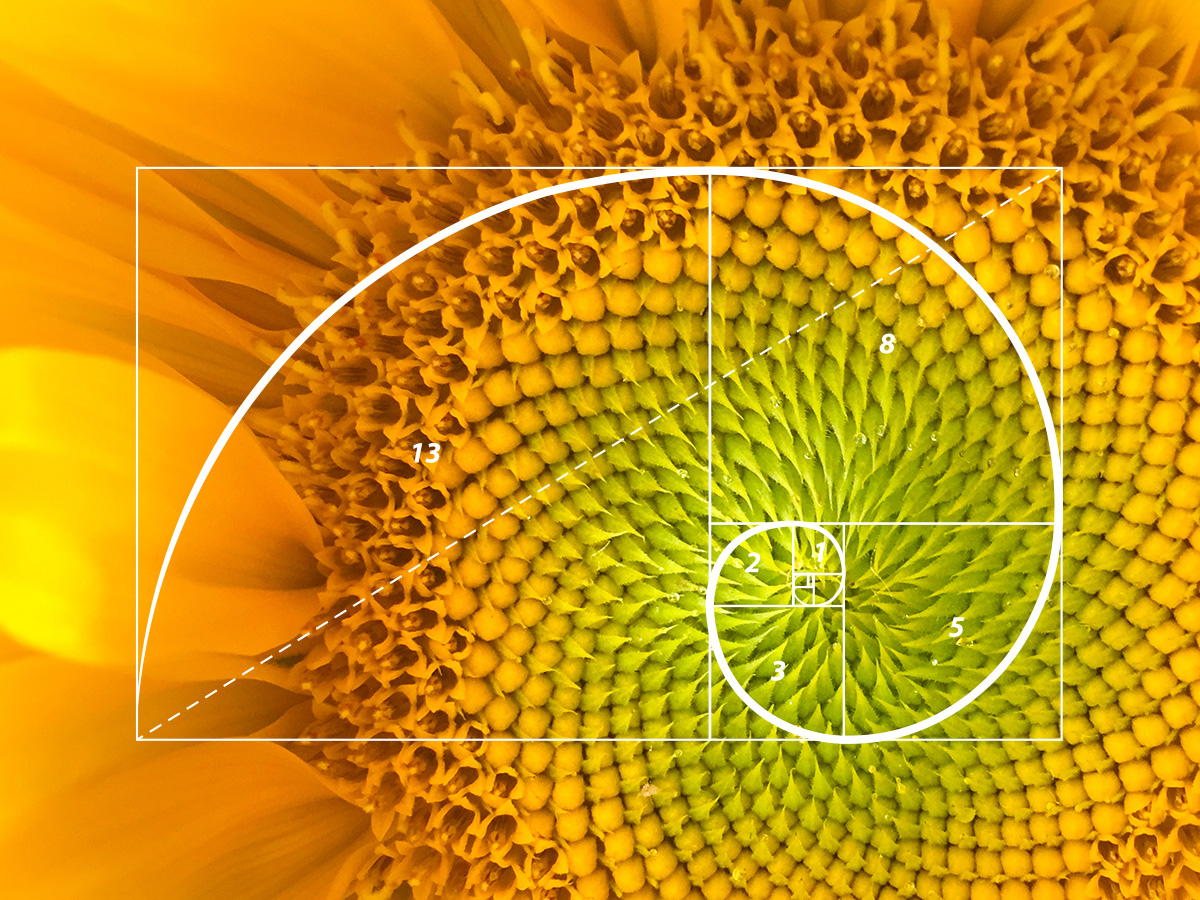
\includegraphics[scale=0.12]{the-golden-ratio-teaser.jpg}
            \end{figure}
        }
    \end{columns}
\end{frame}